%*******************************************************************************
% Example chapter file for books, Copyright A K Peters, Ltd.
%*******************************************************************************
\chapter{Depth of Field with Bokeh Rendering}{Charles de Rousiers and Matt Pettineo}
\label{BokehRendering}

%-------------------------------------------------------------------------------
\section{Introduction}

In order to increase realism and immersion, current games make frequent use of depth of field to simulate lenticular phenomena. Typical implementations use blur based approaches to simulate a camera’s circle of confusion out-of-focus parts of a scene. While such approaches give reasonable results, important features are still missing. In particular, real cameras produce a typical effect that photographers call bokeh (blur in Japanese) appearing at contrasted locations of the final image. Bokeh reveals itself as  bright blurry spots whose shape depends on the camera’s aperture (typically, a circle, a pentagon, or octagon). 

Current and upcoming DirectX11 engines (i.e. Cry engine, Unreal Engine, ...) have recently shown a particular interest for such effects as attested by their most recent demos. Still, it  remains an up-coming technology and precise implementation details are not available yet.

Explicitly drawing the aperture’s shape with quad rendering for every pixel would be rather inefficient. Instead, we propose an hybrid method, mixing previous blur based approaches with quad rendering. Our method selects high contrasted points, and for each of them, renders a quad with an aperture texture. In order to achieve high performance, we use both atomic counters, image texture for random memory access, and indirect draw command for avoiding CPU / GPU synchronizations. This efficient OpenGL 4.2 implementation allows to draw thousands of aperture’s shape at high frame-rate and ensures the temporal coherency of the rendered bokeh.

%-------------------------------------------------------------------------------
\section{Depth of Field Phenomon}\label{Derousiers:DOFPhenomenon}
Depth of field is an important effect to convey realism, especially in opened scenes, with a large field of view. Traditional real-time applications use pinhole camera, which have an infinite depth of field. On the contrary, real camera use thin lens which introduces a limited depth of field. Object outside this depth of field appear blurred on the final image. Object inside this depth of field appear sharp, see Figure~\ref{DeRousiers:focus}.

	\begin{figure}[htb]\centering
	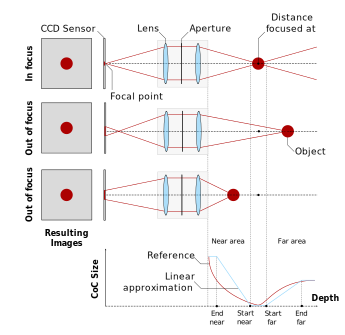
\includegraphics[width=\textwidth]{focus}
	\caption{An object appears blurred depending of its positions in the camera's field of view. 
If an object is in the focused area, then it appear clearly. Othewise, it appears blurred. }
	\label{DeRousiers:focus}
	\end{figure}


The "bluriness" of an object is defined by its circle of confusion (\coc). The size of this \coc depend on the distance to the focused aread. Further a object from focused area is, blurier it appears. The \coc size is not linearly dependent from this distance. It increase faster for the foreground area than for the background area, see Figure~\ref{Derousiers:focus}. \coc depends on focal distance and size lens. It is not obvious to set up the desire depth of field based on those two caracteristics. That is why we use a linear approximation as proposed by~\cite{Hammon07}, see Figure~\ref{DeRousiers:focus}

	\begin{figure}[htb]\centering
	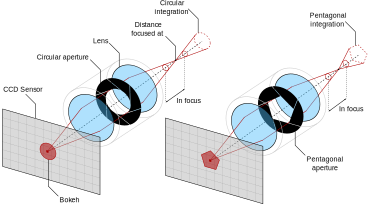
\includegraphics[width=\textwidth]{camera}
	\caption{Aperture's shape of a camera. Aperture's shape modifies pixel integration, and changes bokeh shape }
	\label{DeRousiers:camera}
	\end{figure}

Additionaly, real cameras have an aperture which is in charge to let light come in when a photograph is taken\footnote{If an object or the camera moves during aperture opening, objects will appear blured : it is the motion blur.}. Aperture shape impact directly the final image aspect. Each point out of focus is convolved with the aperture shape. Changing the aperture shape, modify the final image~\ref{DeRousiers:camera}.

While it is hard to see bokeh for low constrated area, bokehs appear clearly for highly constrasted point. We use this observation in our method to optimise performances.

%-------------------------------------------------------------------------------
\section{Relative Work}\label{Derousiers:RelativeWork}

Several methods have been proposed during the last decade to approximate depth of field efficiently. But those methods use gaussian blur or heat diffusion to process unfocused areas~\cite{Kosloff07,Hammon07} and are not able to reproduce bokeh effects.

The earlier approach from Krivanek~\cite{Krivanek03} use sprite splatting for rendering depth of field effect. While this brute force method would allow to render bokehs, it is quite inefficient due to overdraw. Video game industry has shown a recent interest for bokeh effects~\cite{Sousa11,Futurmark11,Mittring11}. While implementation details are uncovered, all those methods seem use a sprite for each pixel, but use clever tricks to optimize performances (hierarchical rasterisation,...). 

A recent approach proposed by White~\cite{White11} reproduce pentagonal bokeh efficiently using several directional blur pass. While efficient, this method does not support arbitrary bokeh shape

%-------------------------------------------------------------------------------
\section{Algorithm}
We observe that only high constrasted points produce distinct bokehs. We use this heuristic to detect bokeh positions in screen space~\cite{Pettineo11} and render final bokehs by splatting textured quad at those locations.

\subsection{Overview}
Our approch is divide into four passes. The first pass computes the circle of confusion size for each pixel based on the depth value of each pixel. The 
Presentation of the overall pipeline

	\begin{figure}[htb]\centering
	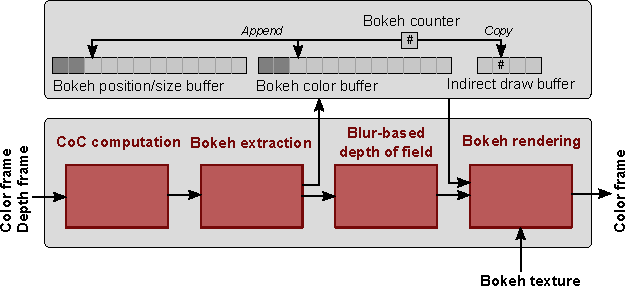
\includegraphics[width=\textwidth]{pipeline}
	\caption{Overview of the pipeline.}
	\label{YourName:fig1}
	\end{figure}

\subsection{Circles of confusion computation}
Settings field of view with focal length is not easy.
We define two areas where geometry is unfocused : a foreground area and a background area.

Both areas are delimited with a near and far depth values. Blur amout is linearly interpolated between those bounds. It allows a easy and intuitive way to set up field of view.

This amount of blur is normalized between [0,1]. An extra parameter MaxRadius determine a posterori what is final size of the blur.
This allows to control both the final apperance but also performances (lesser the maxradius is, greater the performances are).


\subsection{Bokeh detection}
This pass aims to detect pixels which will generate \bokehs. To detect them we use the following heuristic : an highly constrasted point in a given neighborhood will generate a bokeh.
We compare the current pixel valur to the average of it neighborhood. If the current pixel is brighter than a given threshold, then it is register as a bokeh.

In general, only few pixel are detected as \bokeh in comparison to the frame size. The using 
Pixels detected as bokeh are sparse. Storing them into a render target texture would be a waste of space and reading them back would be a waste of time due to their no-coherency in space.

To address this problem, we use \opengl \codecmd{ImageBuffer}s in combinaison with atomic cound. This allows us to built a vector in which we append detected bokehs.

\codecmd{ImageBuffer}s have to be preallocated with a certain size (\ie the maximum number of bokehs which can be display on screen).

The atomic counter store the number of appended bokeh. It uses for know what is the next free cells in the vector.

The two ImageBuffer allows to store size, position, and color of the register bokeh. 


\begin{lstlisting}[language=C++,float={htb},caption={Initialization and drawing for extracting bokehs.},label={YourName:bokehextraction}]

		// Indirect buffer definition
		struct DrawArraysIndirectCommand
		{
			GLuint count;
			GLuint primCount;
			GLuint first;
			GLuint reservedMustBeZero;
		};

		...

		// Create atomic counter
		GLuint indirectBufferID;
		glGenBuffers(1,&indirectBufferID);
		glBindBuffer(GL_DRAW_INDIRECT_BUFFER,indirectBufferID);
		DrawArraysIndirectCommand indirectCmd;
		indirectCmd.count              = 1;
		indirectCmd.primCount          = 6;
		indirectCmd.first              = 0;
		indirectCmd.reservedMustBeZero = 0;
		glBufferData(GL_DRAW_INDIRECT_BUFFER,sizeof(DrawArraysIndirectCommand),&indirecCmd,GL_DYNAMIC_DRAW);

		// Create a texture proxy for the indirect buffer
		glGenTextures(1, &bokehCountTexID);
		glBindTexture(GL_TEXTURE_BUFFER, bokehCountTexID);
		glTexBuffer(GL_TEXTURE_BUFFER, GL_R32UI, pointIndirectBuffer.id);

		// Create position and color textures with a GL_RGBA32F inner format

		...

		// Bind atomic counter
		glActiveTexture(GL_TEXTURE0 + bokehCountTexUnit);
		glBindTexture(GL_TEXTURE_BUFFER, bokehCountTexID);
		glBindImageTexture(bokehCountTexUnit,bokehCountTexID,0,false,0,GL_READ_WRITE,GL_R32UI);

		// Bind position image buffer
		glActiveTexture(GL_TEXTURE0 + bokehPosTexUnit);
		glBindImageTexture(bokehPosTexUnit,bokehPosTex.id,0,false,0,GL_READ_WRITE,GL_RGBA32F);

		// Bind color image buffer
		glActiveTexture(GL_TEXTURE0 + bokehColorTexUnit);
		glBindImageTexture(bokehColorTexUnit,bokehColorTex.id,0,false,0,GL_READ_WRITE,GL_RGBA32F);

		DrawSceenQuad();
\end{lstlisting}


\begin{lstlisting}[language=GLSL,float={htb},caption={Fragment shader for extracting bokehs.},label={YourName:listing1}]
	#version 420

	// Bokeh counter, position (x,y,z,size), and color
	layout(size1x32) coherent uniform uimage1D 	BokehCountTex;
	layout(size4x32) coherent uniform  image1D 	BokehPosTex;
	layout(size4x32) coherent uniform  image1D 	BokehColorTex;

	// Constrast threshold
	uniform float lumThreshold;

	...

	float sizeCenter; // Current CoC size
	vec3 colorCenter; // Current pixel color
	vec3 colorNeighs; // Average color of the neighborhood

	// Append pixel whose constrast is greater than the user's threshold
	float lumNeighs = dot(colorNeighs, vec3(0.299f, 0.587f, 0.114f));
	float lumCenter = dot(colorCenter, vec3(0.299f, 0.587f, 0.114f));
	if((lumCenter-lumNeighs)>lumThreshold)
	{
		int current = int(imageAtomicAdd(BokehCountTex, 1, 1));
		imageStore(BokehPosTex,current,vec4(gl_FragCoord.x,gl_FragCoord.y,gl_FragCoord.z,sizeCenter));
		imageStore(BokehColorTex,current,vec4(colorCenter,1));
	}
\end{lstlisting}


\subsection{Blur-based depth of field}
We do not detail specific approch. Three different approachs are possible : 
\begin{itemize}
	\item Gaussian blur at different resolution + linear blending
	\item Poisson disc sampling + rotation // need lot of sample
	\item Bilateral filtering with variable radius // better
\end{itemize}

The last one offer a good compromise between quality and performance. However it need large radius. A \opencl implementation allows better performances, since shared memory can be used to cache texture fetches.

Depend on quality and performances requested
We refer to previous techniques for this part.

\subsection{Bokeh rendering}

In order to avoir CPU/GPU synchonization, we use an indirect drawing command. \opengl provide the \codecmd{glDrawArraysIndirectInstanced}, which read the number of objects to draw from a indirect buffer. In our case, we read this number from the \codecmd{BokehCounter} buffer.

Simple point are drawn and 
The vertex shader read from \codecmd{BokehPositionBuffer} and \codecmd{BokehColorBuffer} the position and the color of the current \bokeh. Data are read based on their \codecmd{InstanceID}
They are expanded to quad in a geometry shader
The pixel shader read \bokeh's texture



\begin{lstlisting}[language=C++,float={htb},caption={Your caption.},label={YourName:listing1}]

	// Create point VBO
	GLuint pointVboID;
	glm::vec3 defaultPosition(0,0,0);
	glGenBuffers(1,&pointVboID);
	glBindBuffer(GL_ARRAY_BUFFER,pointVboID);
	glBufferData(GL_ARRAY_BUFFER,sizeof(glm::vec3),&defaultPosition,GL_STATIC_DRAW);

	// Create point VAO
	GLuint pointVaoID;
	glGenVertexArrays(1, &pointVaoID);
	glBindVertexArray(pointVaoID);
	glVertexAttribPointer(semantic::PositionLocation,3, GL_RGB,false,GL_FLOAT,GLF_BUFFER_OFFSET(_offset));
	glEnableVertexAttribArray(semantic::PositionLocation);
	glBindBuffer(GL_ARRAY_BUFFER, 0);
	glBindVertexArray(0);

	...

	glMemoryBarrier(GL_ALL_BARRIER_BITS);
	glUseProgram(bokehRenderingProgramID);

	glActiveTexture(GL_TEXTURE0 + bokehShapeTexUnit);
	glBindTexture(GL_TEXTURE_1D,bokehShapeTexID);
	glActiveTexture(GL_TEXTURE0 + bokehColorTexUnit);
	glBindTexture(GL_TEXTURE_1D,bokehColorTexID);
	glActiveTexture(GL_TEXTURE0 + bokehPosTexUnit);
	glBindTexture(GL_TEXTURE_1D,bokehPosTexID);

	glBindVertexArray(pointVaoID);
		glBindBuffer(GL_DRAW_INDIRECT_BUFFER,indirectBufferID);
		glDrawArraysIndirect(GL_POINTS,NULL);
		glBindBuffer(GL_DRAW_INDIRECT_BUFFER,0);
	glBindVertexArray(0);

\end{lstlisting}


\begin{lstlisting}[language=C++,float={htb},caption={Vertex shader for rendering bokeh.},label={YourName:listing1}]
#version 420

uniform vec2      PixelScale;    // (1/xResolution,1/yResolution)
uniform sampler1D BokehPosTex;   // (x,y,z,scale)
uniform sampler1D BokehColorTex;
in vec3           Position;
out float         Radius;
out vec4          Color;

int main()
{
	vec3 pos     = texelFetch(BokehPosTex,gl_InstanceID,0).xyzw;
	Radius       = pos.w;
	Color        = texelFetch(BokehColorTex,gl_InstanceID,0);
	gl_Position	 = vec4( (Position.xy+pos.xy)*PixelScale,pos.z,1);
}
\end{lstlisting}

\begin{lstlisting}[language=GLSL,float={htb},caption={Geometry shader for rendering bokeh.},label={YourName:listing1}]
#version 420

uniform mat4     Transformation;
uniform vec2     PixelScale;
in  float        Radius[1];
in  vec4         Color[1];
out vec4         Radiance;
out vec2         TexCoord;
layout(points)   in;
layout(triangle_strip, max_vertices = 6) out;

void main()
{
	gl_Layer     = 0;
	vec4 offsetx = vec4(PixelScale.x*Radius[0],0,0,0);
	vec4 offsety = vec4(0,PixelScale.y*Radius[0],0,0);
	Radiance     = Color[0];

	// First triangle
	gl_Position = Transformation * ( gl_in[0].gl_Position-offsetx-offsety);
	TexCoord    = vec2(0,0);
	EmitVertex();

	gl_Position = Transformation * ( gl_in[0].gl_Position+offsetx-offsety);
	TexCoord    = vec2(1,0);
	EmitVertex();

	gl_Position = Transformation * ( gl_in[0].gl_Position+offsetx+offsety);
	TexCoord    = vec2(1,1);
	EmitVertex();
	EndPrimitive();

	// Second triangle
	gl_Position = Transformation * ( gl_in[0].gl_Position-offsetx-offsety);
	TexCoord    = vec2(0,0);
	EmitVertex();

	gl_Position = Transformation * ( gl_in[0].gl_Position+offsetx+offsety);
	TexCoord    = vec2(1,1);
	EmitVertex();

	gl_Position = Transformation * ( gl_in[0].gl_Position-offsetx+offsety);
	TexCoord    = vec2(0,1);
	EmitVertex();
	EndPrimitive();
}
\end{lstlisting}

\begin{lstlisting}[language=GLSL,float={htb},caption={Fragment shader for rendering bokeh.},label={YourName:listing1}]
#version 420

uniform sampler2D    BokehShapeTex; // Bokeh shape texture
uniform float        Attenuation;   // Factor for attenuating bokeh borders
in  vec4             Radiance;
in  vec2             TexCoord;
out vec4             FragColor;

void main()
{
	// Add an attenuation function in order to avoid hard edge on the 
	// aperture shape
	float val = textureLod(BokehShapeTex,TexCoord,0).x;
	float att = clamp(length(2.f*(TexCoord-vec2(0.5))),0.f,1.f);
	att       = 1.f - pow(att,Attenuation);
	FragColor = vec4(Radiance.xyz * val * att,Radiance.w);
}
\end{lstlisting}


%-------------------------------------------------------------------------------
\section{Results}

\subsection{Rendering}
	\begin{figure}[htb]\centering
	
\includegraphics[width=\textwidth]{todo}
	\caption{Rendering 1.}
	\label{YourName:fig1}
	\end{figure}

	\begin{figure}[htb]\centering
	
\includegraphics[width=\textwidth]{todo}
	\caption{Rendering 2.}
	\label{YourName:fig1}
	\end{figure}

\subsection{Performances}
	\begin{figure}[htb]\centering
	
\includegraphics[width=\textwidth]{todo}
	\caption{Performances.}
	\label{YourName:fig1}
	\end{figure}

%-------------------------------------------------------------------------------
\section{Discussion}
Temporal coherence and sub-pixel Aliasing
Pre-allocation of a large chunk of memory

%-------------------------------------------------------------------------------
\section{Conclusion}
Sum up

\textbf{Future work:} Several improvments would be done in order to improve performances. 
\begin{itemize}
	\item \textbf{Tile-version} : divide screen into four part and set one atomic-counter per part
	\item \textbf{Mipmap-rasterization} : rasterize bokeh at proper resolution (as done in 3DMark11)
\end{itemize}

%-------------------------------------------------------------------------------
\bibliographystyle{akpbib}
\bibliography{BokehRendering}











